
\parindent=1cm

\section{Сверхновые с коллапсом ядра и формирование нейтронных звезд. Ключевые параметры
нейтронных звезд.}

\subsection{Сверхновые с коллапсом ядра}
Одним из двух типов сверхновых будет сверхновая с коллапсом ядра. В этом случае энергия высвобождается за счет коллапса ядра массивной звезды. В зависимости от того, теряет ли звезда водородную оболочку, сверхновые делятся на два типа.

\begin{figure}[H]
\centering
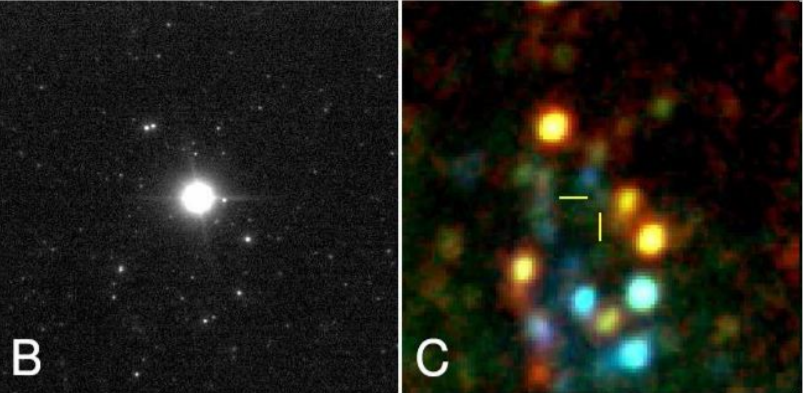
\includegraphics[width=0.7\linewidth]{11_1.png}
\caption{B - сверхновая без водородных линий, C - сверхновая с остатками водородной оболочки}
\label{ЛЕЙБЛ ДЛЯ ССЫЛКИ НА КАРТИНКУ}
\end{figure}

В случае сверхновой с коллапсом звезды -- начальный этап: ядро звезды размером десятки тысяч километров. Далее происходит сжатие ядра до нейтронной звезды с характерным размером около 10 км. Характерная энергия взрыва: $\frac{GM^2}{r} \sim 10^{53}$ эрг , M -  масса ядра (приблизительно равна массе Солнца), r - радиус нейтронной звезды. 

\begin{figure}[H]
\centering
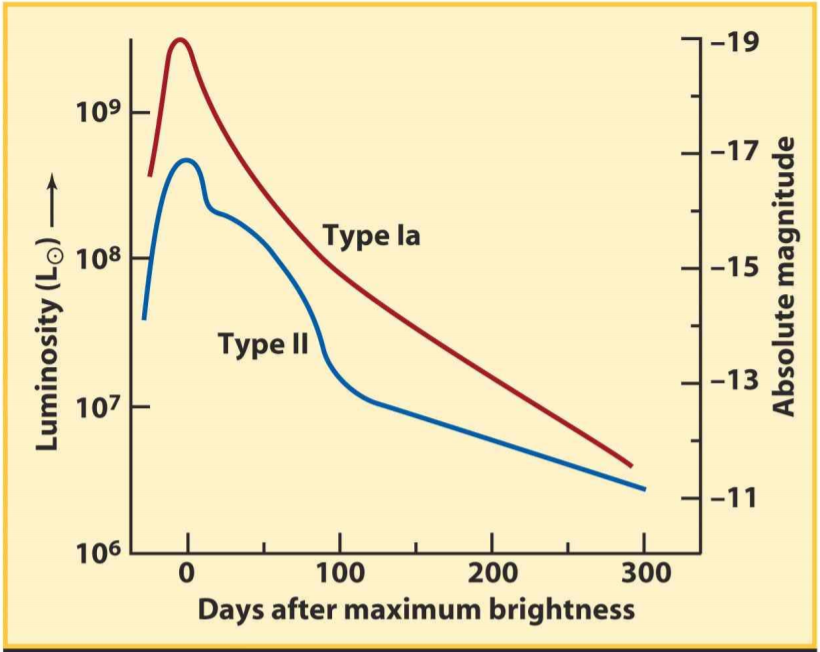
\includegraphics[width=0.6\linewidth]{11_2.png}
\caption{Кривая блеска сверхновой}
\label{ЛЕЙБЛ ДЛЯ ССЫЛКИ НА КАРТИНКУ}
\end{figure}


Максимум блеска достигается при движении ударной волны к поверхности звезды в результате взрыва. Максимум быстро спадает, спустя сотню дней после коллапса сверхновая может быть видна за счет распада радиоактивных элементов. 



В роли переносчика энергии, который будет уносить высвобождающуюся энергию, не взаимодействуя с веществом, выступает нейтрино. Они будут образовываться в результате процесса нейтронизации:

\begin{equation*}
    ^3He + e \rightarrow ^3H + \nu_e
\end{equation*}

\begin{equation*}
    ^4He + e \rightarrow ^3H + n + \nu_e
\end{equation*}

\begin{equation*}
    ^ {56}Fe + e \rightarrow ^{56}Mn + \nu_e
\end{equation*}

За счет этих реакций уносится около 10\% энергии. Оставшаяся часть реализуется за счет так называемого нейтринного охлаждения:

\begin{equation*}
    e^+ +  n \rightarrow \widetilde{\nu_e} + p
\end{equation*}

\begin{equation*}
    e^- + p \rightarrow \nu_e + n
\end{equation*}

Вместо протонов и нейтронов могут выступать и атомные ядра с образованием нестабильного изотопа, который испытывает бета-распад.

\begin{equation*}
    e^- +  (A,Z) \rightarrow (A,Z-1) + \nu_e 
\end{equation*}

\begin{equation*}
    (A,Z-1) \rightarrow (A,Z) + e^- + \widetilde{\nu_e}
\end{equation*}



\subsection{Формирование нейтронных звезд}

Любая звезда главной последовательности с начальной массой, более чем в 8 раз превышающей массу Солнца может в процессе эволюции превратиться в нейтронную звезду. По мере эволюции звезды в её недрах выгорает весь водород, и звезда сходит с главной последовательности. Некоторое время энерговыделение в звезде обеспечивается синтезом более тяжёлых ядер из ядер гелия, но этот синтез заканчивается после того, как все более лёгкие ядра превратятся в ядра с атомным номером, близким к атомному номеру железа — элементам с наибольшей энергией связи ядер.

Когда все ядерное топливо в активной зоне израсходовано, активная зона поддерживается от гравитационного сжатия только давлением вырожденного электронного газа.

При дальнейшем сжатии внешних слоёв звезды, где ещё продолжаются термоядерные реакции синтеза, по мере выгорания лёгких ядер сжатие ядра звезды увеличивается, и масса ядра звезды начинает превышать предел Чандрасекара. Давление вырожденного электронного газа становится недостаточным для поддержания гидростатического равновесия, и ядро начинает быстро уплотняться, в результате чего его температура поднимается выше $5\cdot10^9$ K. При таких температурах происходит фотодиссоциация ядер железа на альфа-частицы под действием жёсткого гамма-излучения. При последующем увеличении температуры происходит слияние электронов и протонов в нейтроны в процессе электронного захвата. В соответствии с законом сохранения лептонного заряда при этом образуется мощный поток электронных антинейтрино.

Когда плотность звезды достигает ядерной плотности $4\cdot10^{17}$ кг/м$^3$, давление вырожденного нейтронного Ферми-газа останавливает сжатие. Падение внешней оболочки звезды на нейтронное ядро останавливается, и она отбрасывается от ядра звезды потоком нейтрино, так как при очень высоких температурах в схлопывающейся оболочке вещество оболочки становится непрозрачным для нейтрино, при этом звезда превращается в сверхновую. После рассеивания внешней оболочки от звезды остаётся звёздный остаток — нейтронная звезда.

По мере того, как ядро массивной звезды сжимается во время взрыва сверхновой II типа, сверхновой Ib типа или Ic типа и коллапсирует в нейтронную звезду, она сохраняет большую часть своего исходного углового момента. Но поскольку радиус остатка звезды во много раз меньше радиуса родительской звезды, момент инерции остатка резко уменьшается, и в соответствии с законом сохранения момента импульса нейтронная звезда приобретает очень высокую угловую скорость вращения, которая постепенно уменьшается в течение очень длительного времени. Известны нейтронные звезды с периодами вращения от 1,4 мс до 30 мс.

Высокая скорость вращения является маркером для обнаружения нейтронных звезд.


\begin{figure}[H]
\centering
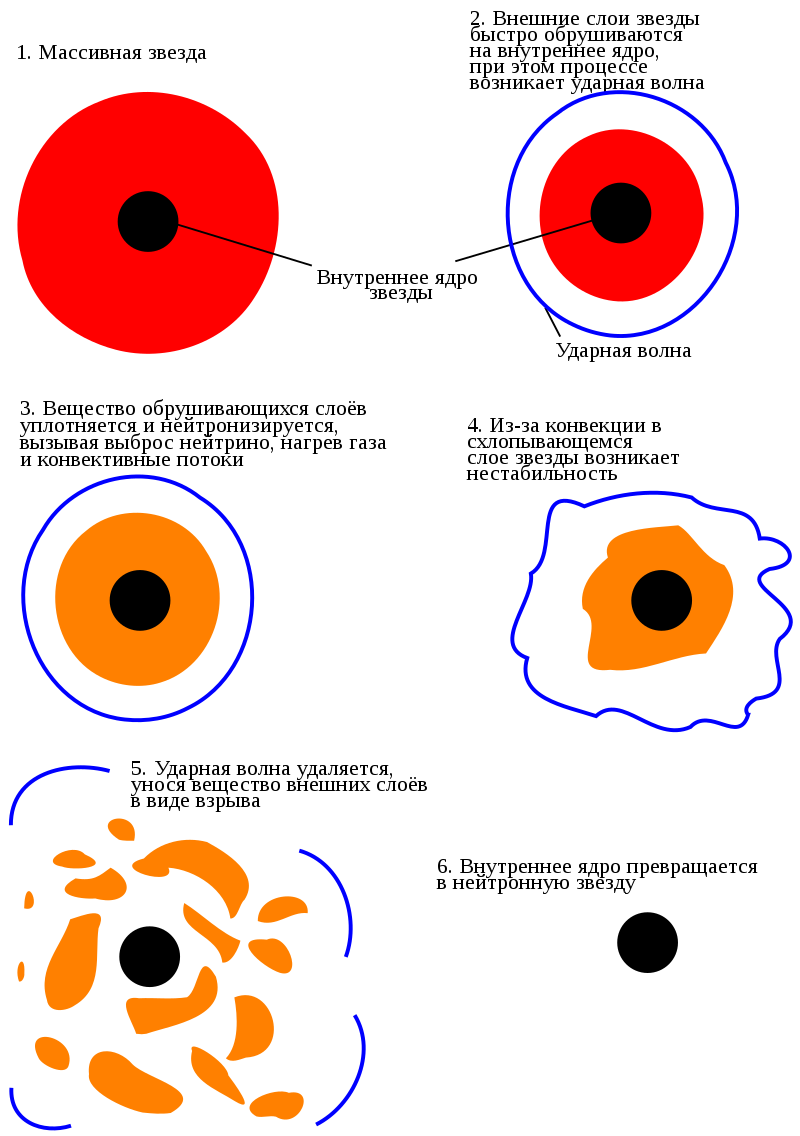
\includegraphics[width=0.6\linewidth]{11_3.png}
\caption{Схема формирования нейтронной звезды}
\label{ЛЕЙБЛ ДЛЯ ССЫЛКИ НА КАРТИНКУ}
\end{figure}




Попов:

Нейтронные звезды также могут быть образованы в результате коллапса белых карликов. При достижении предельной массы (предел Чандрасекара), белый карлик превращается в нейтронную звезду. Гравитационная масса нейтронной зыезды будет меньше массы первоначального белого карлика за счет отвода энергии потоком нейтрино. 




\subsection{Ключевые параметры нейтронных звёзд}

Минимальная масса нейтронной звезды около 1.1 $M_\odot$. Типичная масса: 1.5-2 $M_\odot$. 

$R \sim 9-12$ км. Максимальная масса (при достижении которой нейтронная звезда коллапсирует в черную дыру) -- чуть меньше 2.5 $M_\odot$.

Теоретически возможные нейтронные звезды минимальной массы имеют параметры: $M \sim 0.1 M_\odot, R \sim 250 $ км.

\medskip

\subsection{Типы молодых нейтронных звезд: }

\subsubsection{Магнитары}

Магнитары - нейтронные звезды, чья активность в основном связаана с выделением энергии магнитного поля. Основными кандидатами в магнитары являются аномальные рентгеновские пульсары и источники мягких повторяющихся гамма-всплесков. Порядок магнитного поля: $10^{14}-10^{15}$ Гс.

\subsubsection{Эжекторы (радиопульсары)}
Сильные магнитные поля и малый период вращения. В простейшей модели магнитосферы, магнитное поле вращается твердотельно, то есть с той же угловой скоростью, что и тело нейтронной звезды. На определённом радиусе $ R_{L}=c\omega$ линейная скорость вращения поля приближается к скорости света. Этот радиус называется «радиусом светового цилиндра». За этим радиусом обычное дипольное магнитное поле существовать не может, поэтому линии напряжённости поля в этом месте обрываются. Заряженные частицы, двигающиеся вдоль силовых линий магнитного поля, через такие обрывы могут покидать нейтронную звезду и улетать в межзвёздное пространство. Нейтронная звезда данного типа «эжектирует» (от англ. eject — извергать, выталкивать) релятивистские заряженные частицы, которые излучают в радиодиапазоне. Эжекторы наблюдаются как радиопульсары.
\subsubsection{"Пропеллер"}

Скорость вращения уже недостаточна для эжекции частиц, поэтому такая звезда не может быть радиопульсаром. Однако скорость вращения всё ещё велика, и захваченное магнитным полем окружающее нейтронную звезду вещество не может упасть на поверхность, то есть аккреция вещества не происходит. Нейтронные звёзды данного типа практически не наблюдаемы и изучены плохо.

\subsubsection{Аккреторы (рентгеновские пульсары)}

Скорость вращения снижается настолько, что веществу теперь ничего не препятствует падать на такую нейтронную звезду. Падая, вещество, уже будучи в состоянии плазмы, движется по линиям магнитного поля и ударяется о поверхность тела нейтронной звезды в районе её полюсов, разогреваясь при этом до десятков миллионов градусов. Вещество, нагретое до столь высоких температур, ярко светится в мягком рентгеновском диапазоне. Размер области, в которой происходит столкновение падающего вещества с поверхностью тела нейтронной звезды, очень мала — всего около 100 метров. Это горячее пятно из-за вращения звезды периодически затмевается телом звезды, поэтому наблюдаются регулярные пульсации рентген-излучения. Такие объекты и называются рентгеновскими пульсарами.

\subsubsection{Георотатор}

Скорость вращения таких нейтронных звёзд мала и не препятствует аккреции. Но размеры магнитосферы таковы, что плазма останавливается магнитным полем раньше, чем она будет захвачена гравитацией. Подобный механизм работает в магнитосфере Земли, из-за чего данный тип нейтронных звёзд и получил своё название.


